\documentclass[../../main-ap-physics.tex]{subfiles}

\begin{document}

\section{Two-Dimensional Kinematics}

\subsection{Kinematics in Two Dimensions: An Introduction}

\subsubsection*{Two-Dimensional Motion: Walking in a City}

Suppose you want to walk from one point to another in a city with uniform square blocks, as pictured in Figure \ref{5wAnWT}

\begin{center}
    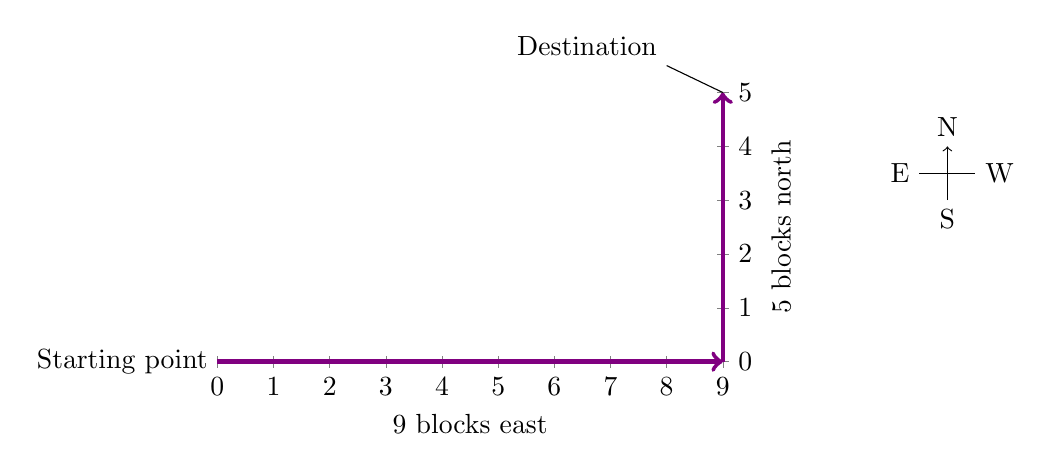
\begin{tikzpicture}
        \begin{axis}[width=8cm, height=5cm,
            xmin=0,xmax=9,
            ymin=0,ymax=5,
            xtick={0,1,...,9},
            ytick={0,1,...,5},
            clip=false,
            axis y line = right,
            axis x line = left,
            xlabel={9 blocks east},
            ylabel={5 blocks north},
        ]
        \draw[->,ultra thick,violet] (0,0) -- (9,0);
        \draw[->,ultra thick,violet] (9,0) -- ++(0,5);
        \node[left] at (0,0) {Starting point};
        \draw (9,5) -- ++(-1,0.5) node[above left] {Destination};
        \begin{scope}[shift={(13,3)}]
            \draw[->] (0,0) node[below] {S} -- ++(0,1) node[above] {N};
            \draw (-0.5,0.5) node[left] {E} -- ++(1,0) node [right] {W};
        \end{scope}
        \end{axis}
    \end{tikzpicture}
    \captionsetup{type=figure,margin=1in,font=scriptsize}
    \captionof{figure}{A pedestrian walks a two-dimensional path between two points in a city. In this scene, all blocks are square and are the same size.}
    \label{5wAnWT}
\end{center}

The straight-line path that a helicopter might fly is blocked to you as a pedestrian, and so you are forced to take a two-dimensional path, such as the one shown. You walk 14 blocks in all, 9 east followed by 5 north. What is the straight-line distance?

\vspace{1em}

An old adage states that the shortest distance between two points is a straight line. The two legs of the trip and the straight-line path form a right triangle, and so the Pythagorean theorem,  $a^2 + b^2 = c^2$, can be used to find the straight-line distance.

\begin{equation}
    a^2 + b^2 = c^2
\end{equation}

\begin{center}
    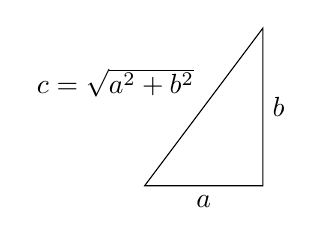
\begin{tikzpicture}
        \draw (0,0) -- (1.5,0) node[pos=0.5,below] {$a$} -- ++(0,2) node[pos=0.5,right] {$b$} -- cycle node[pos=0.5,above left] {$c = \sqrt{a^2 + b^2}$};
    \end{tikzpicture}
    \captionsetup{type=figure,margin=1in,font=scriptsize}
    \captionof{figure}{The Pythagorean theorem relates the length of the legs of a right triangle, labeled $a$ and $b$, with the hypotenuse, labeled $c$. The relationship is given by: $a^2 + b^2 = c^2$. This can be rewritten, solving for $c$: $c = \sqrt{a^2 + b^2}$.}
\end{center}

The hypotenuse of the triangle is the straight-line path, and so in this case its length in units of city blocks is 

\begin{equation*}
    \sqrt{\left(\SI{9}{blocks}\right)^2 + \left(\SI{5}{blocks}\right)^2} = \SI{10.3}{blocks}
\end{equation*}

considerably shorter than the 14 blocks you walked. (Note that we are using three significant figures in the answer. Although it appears that ``9'' and ``5'' have only one significant digit, they are discrete numbers. In this case ``9 blocks'' is the same as ``9.0 or 9.00 blocks.'' We have decided to use three significant figures in the answer in order to show the result more precisely.)

\begin{center}
    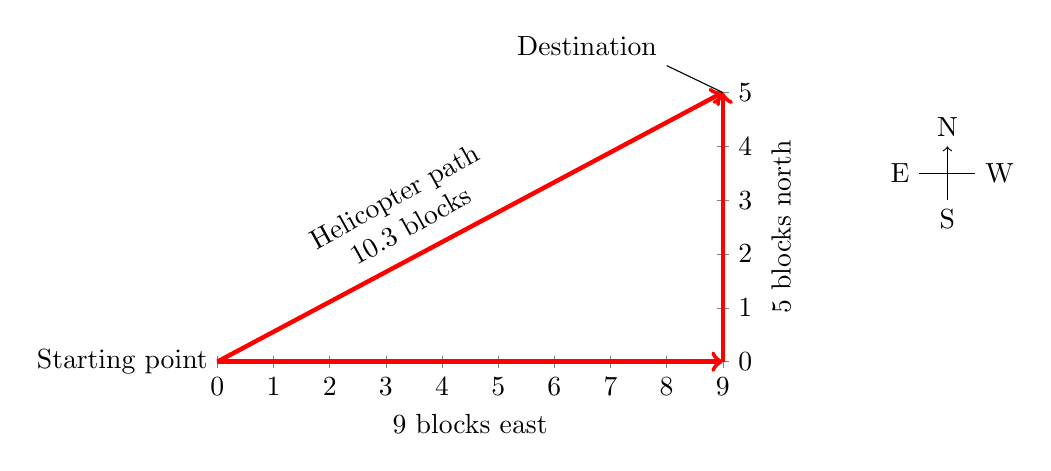
\begin{tikzpicture}
        \begin{axis}[width=8cm, height=5cm,
            xmin=0,xmax=9,
            ymin=0,ymax=5,
            xtick={0,1,...,9},
            ytick={0,1,...,5},
            clip=false,
            axis y line = right,
            axis x line = left,
            xlabel={9 blocks east},
            ylabel={5 blocks north},
        ]
        \draw[->,ultra thick,red] (0,0) -- (9,0);
        \draw[->,ultra thick,red] (9,0) -- ++(0,5);
        \draw[->,ultra thick,red] (0,0) -- (9,5) node[pos=0.6, above left=1mm,rotate=29,align=center,black] {Helicopter path\\10.3 blocks} node[black,below,pos=0.5,rotate=29] {\Large \myheli};
        \node[left] at (0,0) {Starting point};
        \draw (9,5) -- ++(-1,0.5) node[above left] {Destination};
        \begin{scope}[shift={(13,3)}]
            \draw[->] (0,0) node[below] {S} -- ++(0,1) node[above] {N};
            \draw (-0.5,0.5) node[left] {E} -- ++(1,0) node [right] {W};
        \end{scope}
        \end{axis}
    \end{tikzpicture}
    \captionsetup{type=figure,margin=1in,font=scriptsize}
    \captionof{figure}{The straight-line path followed by a helicopter between the two points is shorter than the 14 blocks walked by the pedestrian. All blocks are square and the same size.}
    \label{R2c4pp}
\end{center}

The fact that the straight-line distance (10.3 blocks) in Figure \ref{R2c4pp} is less than the total distance walked (14 blocks) is one example of a general characteristic of vectors. (Recall that vectors are quantities that have both magnitude and direction.)

\vspace{1em}

As for one-dimensional kinematics, we use arrows to represent vectors. The length of the arrow is proportional to the vector's magnitude. The arrow's length is indicated by hash marks in Figure \ref{5wAnWT} and Figure \ref{R2c4pp}. The arrow points in the same direction as the vector. For two-dimensional motion, the path of an object can be represented with three vectors: one vector shows the straight-line path between the initial and final points of the motion, one vector shows the horizontal component of the motion, and one vector shows the vertical component of the motion. The horizontal and vertical components of the motion add together to give the straight-line path. For example, observe the three vectors in Figure \ref{R2c4pp}. The first represents a 9-block displacement east. The second represents a 5-block displacement north. These vectors are added to give the third vector, with a 10.3-block total displacement. The third vector is the straight-line path between the two points. Note that in this example, the vectors that we are adding are perpendicular to each other and thus form a right triangle. This means that we can use the Pythagorean theorem to calculate the magnitude of the total displacement. (Note that we cannot use the Pythagorean theorem to add vectors that are not perpendicular. We will develop techniques for adding vectors having any direction, not just those perpendicular to one another, in ``Vector Addition and Subtraction: Graphical Methods and Vector Addition and Subtraction: Analytical Methods.'')

\subsubsection*{The Independence of Perpendicular Motions}

The person taking the path shown in Figure \ref{R2c4pp} walks east and then north (two perpendicular directions). How far they walk east is only affected by their motion eastward. Similarly, how far they walk north is only affected by their motion northward.

\begin{gradient}{INDEPENDENCE OF MOTION}
    The horizontal and vertical components of two-dimensional motion are independent of each other. Any motion in the horizontal direction does not affect motion in the vertical direction, and vice versa.
\end{gradient}

This is true in a simple scenario like that of walking in one direction first, followed by another. It is also true of more complicated motion involving movement in two directions at once. For example, let's compare the motions of two baseballs. One baseball is dropped from rest. At the same instant, another is thrown horizontally from the same height and follows a curved path. A stroboscope has captured the positions of the balls at fixed time intervals as they fall.

\begin{center}
    \begin{tikzpicture}
        \begin{axis}[width=7cm,height=8cm,ticks=none,
        axis lines = center,
        axis line style={draw=none},
        clip=false,
        xmin=0, xmax=120,
        ymin=0, ymax=70,
        ]
        % \draw[only marks,domain=0:100,variable=\x,samples=200] plot ({\x},{patheq(\x,60,28.6,0)});
        % \draw[dashed] (0,{patheq(0,60,28.6,0)}) -- ++(100,0);
        % \draw[dashed] (0,{patheq(0,60,28.6,0)}) -- ++(0,-{patheq(0,60,28.6,0)});
        
        \pgfplotsinvokeforeach{20,40,60,80,100}{
            \draw[thick,Green,->] (#1,{patheq(#1,60,28.6,0)}) -- ++(0,-0.2*#1);
            \draw[thick,->] (#1,{patheq(#1,60,28.6,0)}) -- ++(15,0);
            \fill[RoyalBlue] (#1,{patheq(#1,60,28.6,0)}) circle (3pt);
            
            \draw[dashed] (0,{patheq(#1,60,28.6,0)}) -- ++(#1,0);

            \draw[thick,Green,->] (0,{patheq(#1,60,28.6,0)}) -- ++(0,-0.2*#1);
            \fill[red] (0,{patheq(#1,60,28.6,0)}) circle (3pt);
        }
        \end{axis}
    \end{tikzpicture}
    \captionsetup{type=figure,margin=1in,font=scriptsize}
    \captionof{figure}{This shows the motions of two identical balls—one falls from rest, the other has an initial horizontal velocity. Each subsequent position is an equal time interval. Arrows represent horizontal and vertical velocities at each position. The ball on the right has an initial horizontal velocity, while the ball on the left has no horizontal velocity. Despite the difference in horizontal velocities, the vertical velocities and positions are identical for both balls. This shows that the vertical and horizontal motions are independent.}
    \label{iZGL98}
\end{center}

It is remarkable that for each flash of the strobe, the vertical positions of the two balls are the same. This similarity implies that the vertical motion is independent of whether or not the ball is moving horizontally. (Assuming no air resistance, the vertical motion of a falling object is influenced by gravity only, and not by any horizontal forces.) Careful examination of the ball thrown horizontally shows that it travels the same horizontal distance between flashes. This is due to the fact that there are no additional forces on the ball in the horizontal direction after it is thrown. This result means that the horizontal velocity is constant, and affected neither by vertical motion nor by gravity (which is vertical). Note that this case is true only for ideal conditions. In the real world, air resistance will affect the speed of the balls in both directions.

\vspace{1em}

The two-dimensional curved path of the horizontally thrown ball is composed of two independent one-dimensional motions (horizontal and vertical). The key to analyzing such motion, called projectile motion, is to resolve (break) it into motions along perpendicular directions. Resolving two-dimensional motion into perpendicular components is possible because the components are independent. We shall see how to resolve vectors in ``Vector Addition and Subtraction: Graphical Methods'' and ``Vector Addition and Subtraction: Analytical Methods.'' We will find such techniques to be useful in many areas of physics.

\begin{gradient}{PHET EXPLORATIONS}
    \textbf{Ladybug Motion 2D}: Learn about position, velocity and acceleration vectors. Move the ladybug by setting the position, velocity or acceleration, and see how the vectors change. Choose linear, circular or elliptical motion, and record and playback the motion to analyze the behavior.

    \vspace{1em}

    \href{https://openstax.org/l/28ladybugmotion}{Click to view content}.
\end{gradient}

\subsection{Vector Addition and Subtraction: Graphical Methods}

\subsubsection*{Vectors in Two Dimensions}

A \gls{vector} is a quantity that has magnitude and direction. Displacement, velocity, acceleration, and force, for example, are all vectors. In one-dimensional, or straight-line, motion, the direction of a vector can be given simply by a plus or minus sign. In two dimensions (2-d), however, we specify the direction of a vector relative to some reference frame (i.e., coordinate system), using an arrow having length proportional to the vector's magnitude and pointing in the direction of the vector.

\vspace{1em}
Figure ?.?? shows such a graphical representation of a vector, using as an example the total displacement for the person walking in a city considered in Kinematics in Two Dimensions: An Introduction. We shall use the notation that a boldface symbol, such as $\mathbf{D}$, stands for a vector. Its magnitude is represented by the symbol in italics, \textbf{\textit{D}}, and its direction by $\theta$.

\begin{gradient}{VECTORS IN THIS TEXT}
    In this text, we will represent a vector with a boldface variable. For example, we will represent the quantity force with the vector $\textbf{F}$, which has both magnitude and direction. The magnitude of the vector will be represented by a variable in italics, such as \textbf{\textit{F}}, and the direction of the variable will be given by an angle $\theta$.
\end{gradient}

\begin{center}
    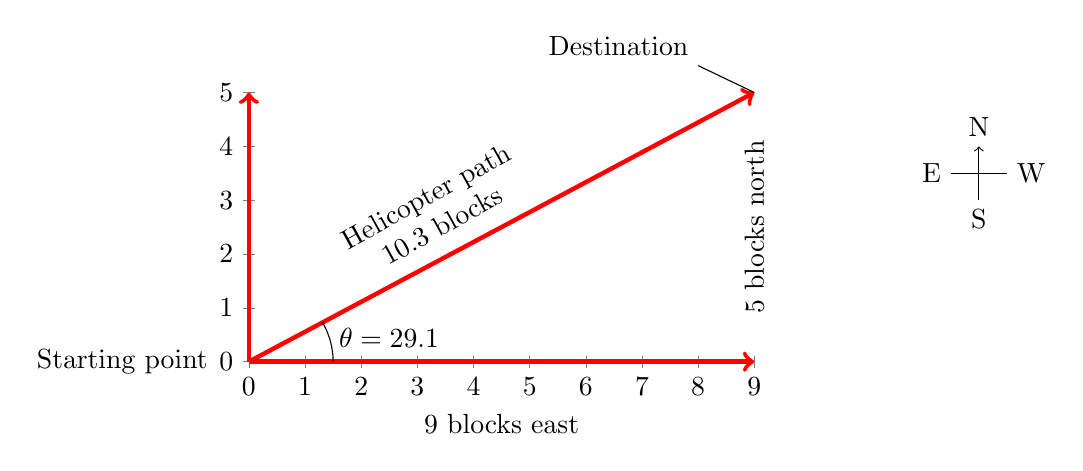
\begin{tikzpicture}
        \begin{axis}[width=8cm, height=5cm,
            xmin=0,xmax=9,
            ymin=0,ymax=5,
            xtick={0,1,...,9},
            ytick={0,1,...,5},
            clip=false,
            axis lines = left,
            xlabel={9 blocks east},
        ]
        \draw[->,ultra thick,red] (0,0) -- (9,0);
        \draw[->,ultra thick,red] (0,0) -- ++(0,5);
        \draw[->,ultra thick,red] (0,0) -- (9,5) node[pos=0.6, above left=1mm,rotate=29,align=center,black] {Helicopter path\\10.3 blocks} node[black,below,pos=0.5,rotate=29] {\Large \myheli};
        \node[left=4mm] at (0,0) {Starting point};
        \draw (9,5) -- ++(-1,0.5) node[above left] {Destination};
        \draw (1.5,0) arc (0:29.1:1.5) node[right,pos=0.6] {$\theta = \ang{29.1}$};
        \node[rotate=90] at (9,2.5) {5 blocks north};
        \begin{scope}[shift={(13,3)}]
            \draw[->] (0,0) node[below] {S} -- ++(0,1) node[above] {N};
            \draw (-0.5,0.5) node[left] {E} -- ++(1,0) node [right] {W};
        \end{scope}
        \end{axis}
    \end{tikzpicture}
    \captionsetup{type=figure,margin=1in,font=scriptsize}
    \captionof{figure}{A person walks 9 blocks east and 5 blocks north. The displacement is 10.3 blocks at an angle \ang{29.1} north of east.}
\end{center}

\begin{center}
    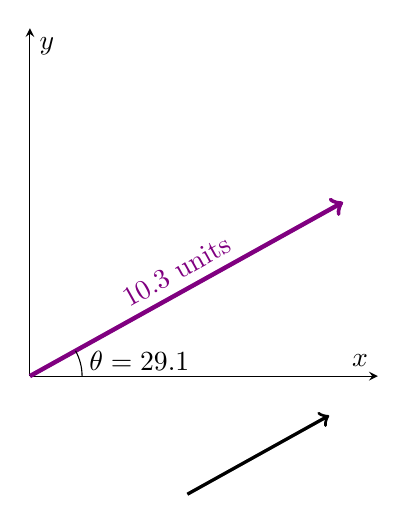
\begin{tikzpicture}
        \begin{axis}[width=6cm,height=6cm,
            xmin=0,xmax=10,
            ymin=0,ymax=10,
            ticks=none,
            axis lines=center,
            xlabel={$x$},
            ylabel={$y$},
            clip=false
        ]
        \draw[ultra thick,violet,->] (0,0) -- ++(9,5) node[pos=0.5,above,rotate=29.1] {10.3 units};
        \draw (1.5,0) arc (0:29:1.5) node[pos=0.6,right] {$\theta = \ang{29.1}$};
        \end{axis}
        \tkzRegle[Fond=true,Opacite=0.9,CouleurFond=yellow,AfficheValeurs=false,Origine={(-0.5,1)},Echelle=0.4,Rotation=29.1]
        \tkzRapporteur[Fond,CouleurFond=blue,Echelle=0.3,Origine={(2,-1.5)},AfficheAngles=false]
        \draw[very thick,->] (2,-1.5) -- ++(0.2*9,0.2*5);
    \end{tikzpicture}
    \captionsetup{type=figure,margin=1in,font=scriptsize}
    \captionof{figure}{To describe the resultant vector for the person walking in a city considered in Figure ?.?? graphically, draw an arrow to represent the total displacement vector $\textbf{D}$. Using a protractor, draw a line at an angle $\theta$ relative to the east-west axis. The length \textbf{\textit{D}} of the arrow is proportional to the vector's magnitude and is measured along the line with a ruler. In this example, the magnitude \textbf{\textit{D}} of the vector is 10.3 units, and the direction $\theta$ is \ang{29.1} north of east.}
\end{center}

\subsubsection*{Vector Addition: Head-to-Tail Method}

The head-to-tail method is a graphical way to add vectors, described in Figure ?.?? below and in the steps following. The tail of the vector is the starting point of the vector, and the head (or tip) of a vector is the final, pointed end of the arrow.

\begin{center}
    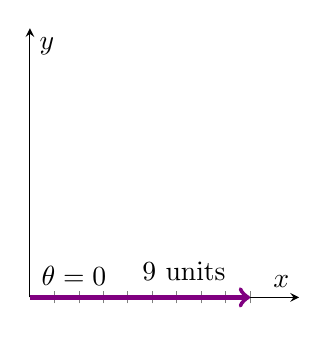
\begin{tikzpicture}
        \begin{axis}[width=5cm,height=5cm,
            xmin=0,xmax=11,
            ymin=0,ymax=11,
            axis lines=center,
            xlabel={$x$},
            ylabel={$y$},
            clip=false,
            xtick={0,1,...,9},
            ytick=\empty,
            xticklabels={},
        ]
        \draw[ultra thick,violet,->] (0,0) -- ++(9,0) node[pos=0.2,above,black] {$\theta = \ang{0}$} node[pos=0.7,above=2pt,black] {9 units};
        \end{axis}
    \end{tikzpicture}%
    \hspace{1em}
        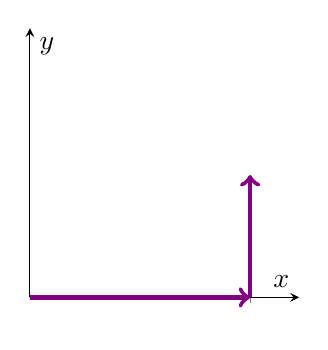
\begin{tikzpicture}
        \begin{axis}[width=5cm,height=5cm,
            xmin=0,xmax=11,
            ymin=0,ymax=11,
            axis lines=center,
            xlabel={$x$},
            ylabel={$y$},
            clip=false,
            xtick={9},
            ytick=\empty,
            xticklabels={},
        ]
        \draw[ultra thick,violet,->] (0,0) -- ++(9,0);
        \draw[ultra thick,violet,->] (9,0) -- ++(0,5);
        \end{axis}
    \end{tikzpicture}
    \captionsetup{type=figure,margin=1in,font=scriptsize}
    \captionof{figure}{}
\end{center}


\end{document}